% This file contains the content for a main section
\numberedformat
%% Modify below this line %%
\chapter{Mapping from the engineering-centric to user-centric terms}

There is not a one-to-one mapping of the RRT to a View Transform or from an ODT to a Display Transform. 

\autoref{fig:conceptualModel} shows the ACES viewing pipeline using the engineering-centric LMT, RRT, and ODT terms. \autoref{fig:userCentricModel} shows how the recommended terms apply to the same underlying blocks being used in \autoref{fig:conceptualModel}. Note that both pipelines produce exactly the same numerical results.

Two new engineering-centric acronyms are used here since there is a need to be able to refer to the part of the ODT which contains the Academy-developed part of the algorithm (which is key to the look of the system), from the more typical conversion from colorimetry into code values for a given display.

Target Conversion Transform (TCT) -- The TCT may be thought of as the part that ``fits'' the idealized colorimetry from the RRT into what is appropriate for a viewing target. A viewing target consists of a family of display devices (i.e. devices which have similar dynamic range and gamut characteristics) and associated viewing environment.

Display Encoding Transform (DET) -- The DET is simply a conversion from colorimetry into the code values necessary to produce that colorimetry on a given device. It is similar to an ICC monitor profile.

\begin{figure}[htbp]
\begin{center}
    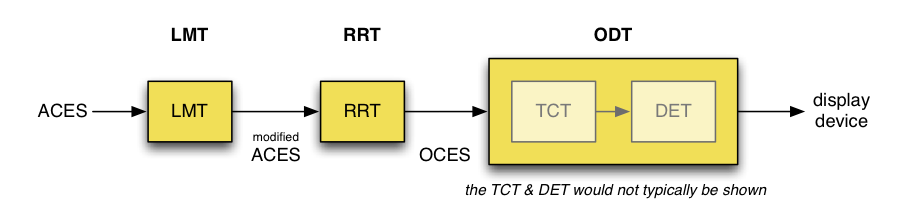
\includegraphics[width=\textwidth]{conceptualModel.png}
\caption{The conceptual model of viewing ACES}
\label{fig:conceptualModel}
\end{center}
\end{figure}

\begin{figure}[htbp]
\begin{center}
    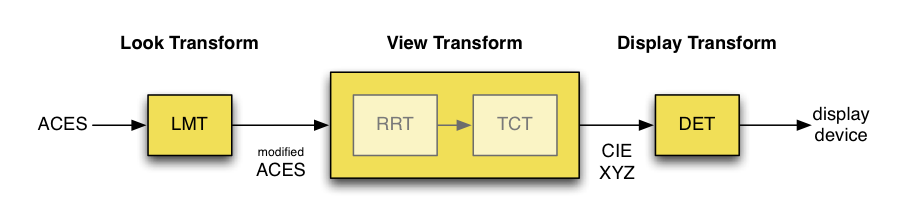
\includegraphics[width=\textwidth]{userCentricModel.png}
\caption{Engineering-centric ACES viewing pipeline along with the user-centric model}
\label{fig:userCentricModel}
\end{center}
\end{figure}
